\documentclass{gshs_poster_beamer}
\usepackage{enumitem}
\usepackage{amsmath, amssymb} % equation
\usepackage{kotex} % korean
\usepackage{graphicx} % to use \includegraphics
\graphicspath{{images/}}
\usepackage{siunitx} % SI unit
\usepackage{subcaption}
\setitemize[1]{label={\raise1.25pt\hbox{$\blacktriangleright$}}}
\setitemize[2]{label={\scriptsize\raise1.25pt\hbox{$\blacktriangleright$}}}
\setitemize[3]{label={\raise1.25pt\hbox{$\star$}}}
\setitemize[4]{label={-}}
%\setenumerate[1]{label={\theenumi.}}
%%% title, authors, etc...
\ptitle{천체망원경 모터 포커서 컨트롤러 구동 시스템 개발 및 ASCOM 드라이버 개발\\[0.3em]}
\authorone{곽지성}
\authortwo{정기현}
\teacher{박기현}

\begin{document}
\pagestyle{fancy}
\maketitle
%\vspace{1em} 

\begin{columns}[T]

%% Left Column
\column{0.3\textwidth}


\begin{posterbox}[colbacktitle=orange!70,coltitle=black,colback=orange!5]{요약}
본 논문에서는 자동 초점 조절 구동 시스템을 구현하기 위한 방법을 제안한다. 자동 초점 조절 구동 펌웨어는 기본적으로 arduino를 사용하며 여러 기능들이 존재하여 자유로운 설정이 가능하다. ASCOM 드라이버는 C\# 코딩을 이용하여 컴퓨터로 정보 전달이 가능하다. 본 논문에서 제안된 방법은 사람이 손으로 제어하는 것보다 정밀하고 빠르게 천체망원경의 초점을 맞출 수 있도록 편의성을 제공한다.
\end{posterbox}

\vspace{1em}

\begin{posterbox}[colbacktitle=magenta!60,coltitle=black,colback=magenta!5]{연구 배경}
\begin{itemize}
	\item 천체망원경의 초점을 사람의 손으로 맞추는 것은 흔들림으로 인하여 쉽지 않다.
	\item 이러한 문제를 해결하기 위하여 'Starizona' 회사에서 자동초점조절 장치인 'Micro Touch'를 개발하였다.
	\item 그러나 이를 사용할 때 여러 가지 불편한 점들이 있고, 가격도 매우 비싸다.
	\item 해결책은 이러한 펌웨어를 더욱 저렴한 가격에 개발하는 것이다.
\end{itemize}
\end{posterbox}

\vspace{1em}

\begin{posterbox}[colbacktitle=black,coltitle=white,colback=black!5]{References}{사용한 물품}
	\begin{itemize}
		\item 천체망원경
		\begin{itemize}
			\item TEC140 광학계에는 Starlight Instruments에서 제작한 3.5" Feather Touch Focuser가 장착 되어 있다.
			\item Starlight Instruments에서는 3.5" Feather Touch Focuser에 장착할 수 있는 STEPPER MOTOR와 MICRO TOUCH FOCUSING SYSTEM을 제작하여 판매하고 있다.
			\item 모터는 구입한 것을 사용하고 MICRO TOUCH FOCUSING SYSTEM과 같은 기능을 가진 포커서 컨트롤러를 제작하였다.
		\end{itemize}
	\begin{figure}[h]
		\centering
		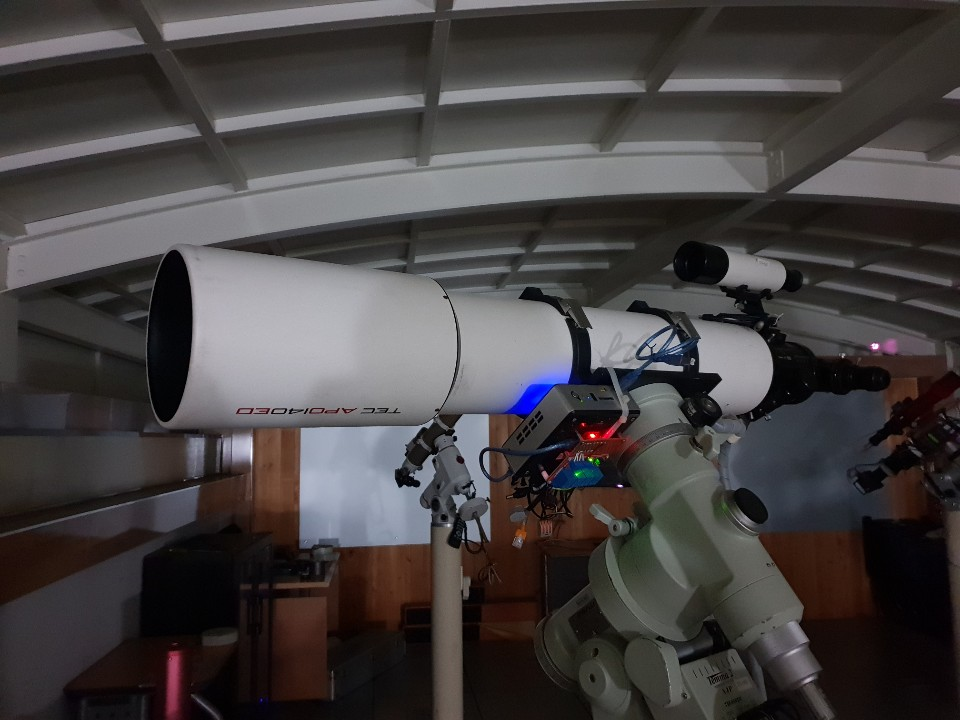
\includegraphics[scale=0.4]{telescope}
		\caption{사용한 천체망원경}
		\label{fig:telescope}
	\end{figure}
		\item arduino
		\begin{itemize}
			\item arduino ARDUINO NANO
			\item 0.96" oled screen I2C
			\item Adafruit Industries 385
			\item Apem MJTP1230B
			\item BP5277-90
			\item HC-05 bluetooth
			\item LED 3mm 90', Ohmite OD473JE
			\item Panasonic EEA-GA1C100H
			\item SparkFun WRL-13678
			\item Sprague 1C10X7R104K050B
			\item TE Connectivity/AMP 5525258-3
			\item TMC2100
			\item Wurth Elektronik 694106301002
		\end{itemize}
	\end{itemize}
\end{posterbox}


%% Center Column
\column{0.3\textwidth}

\begin{posterbox}[colbacktitle=green!50,coltitle=black,colback=green!5]{선행연구 고찰}
	\begin{itemize}
		\item 이덕규 외(2014)는 복합재 광구조체와 결합하여 전자광학카메라의 영상품질을 향상시킬 수 있는 초점조절장치를 개발하였다.\cite{leedukgu2014}
		\item 윤종환 외(2011)는 선명도에 관한 기울기를 이용하여 초점이 맞았는지를 확인하는 방법을 사용하였다.\cite{yunjonghwan2011lcd}
		\item 박석휘 외(2009)는 모바일 폰용 자동 초점 조절 알고리즘을 초점 값 계산 알고리즘을 이용하여 구현하였다.\cite{parksukhui2009Median}
		\item 이성희 외(1998)는 각 화소들의 미디언 값의 차이를 이용하여 초점을 맞추는 알고리즘을 구현하였다.\cite{leeseonghee1998Median}
	\end{itemize}
\end{posterbox}

\vspace{1em}

\begin{posterbox}[colbacktitle=blue!50!black,coltitle=white,colback=cyan!5]{개발 내용 및 방법}
  \begin{itemize}
	\item 모터 포커서 컨트롤러 회로 설계
	\begin{figure}[h]
		\centering
		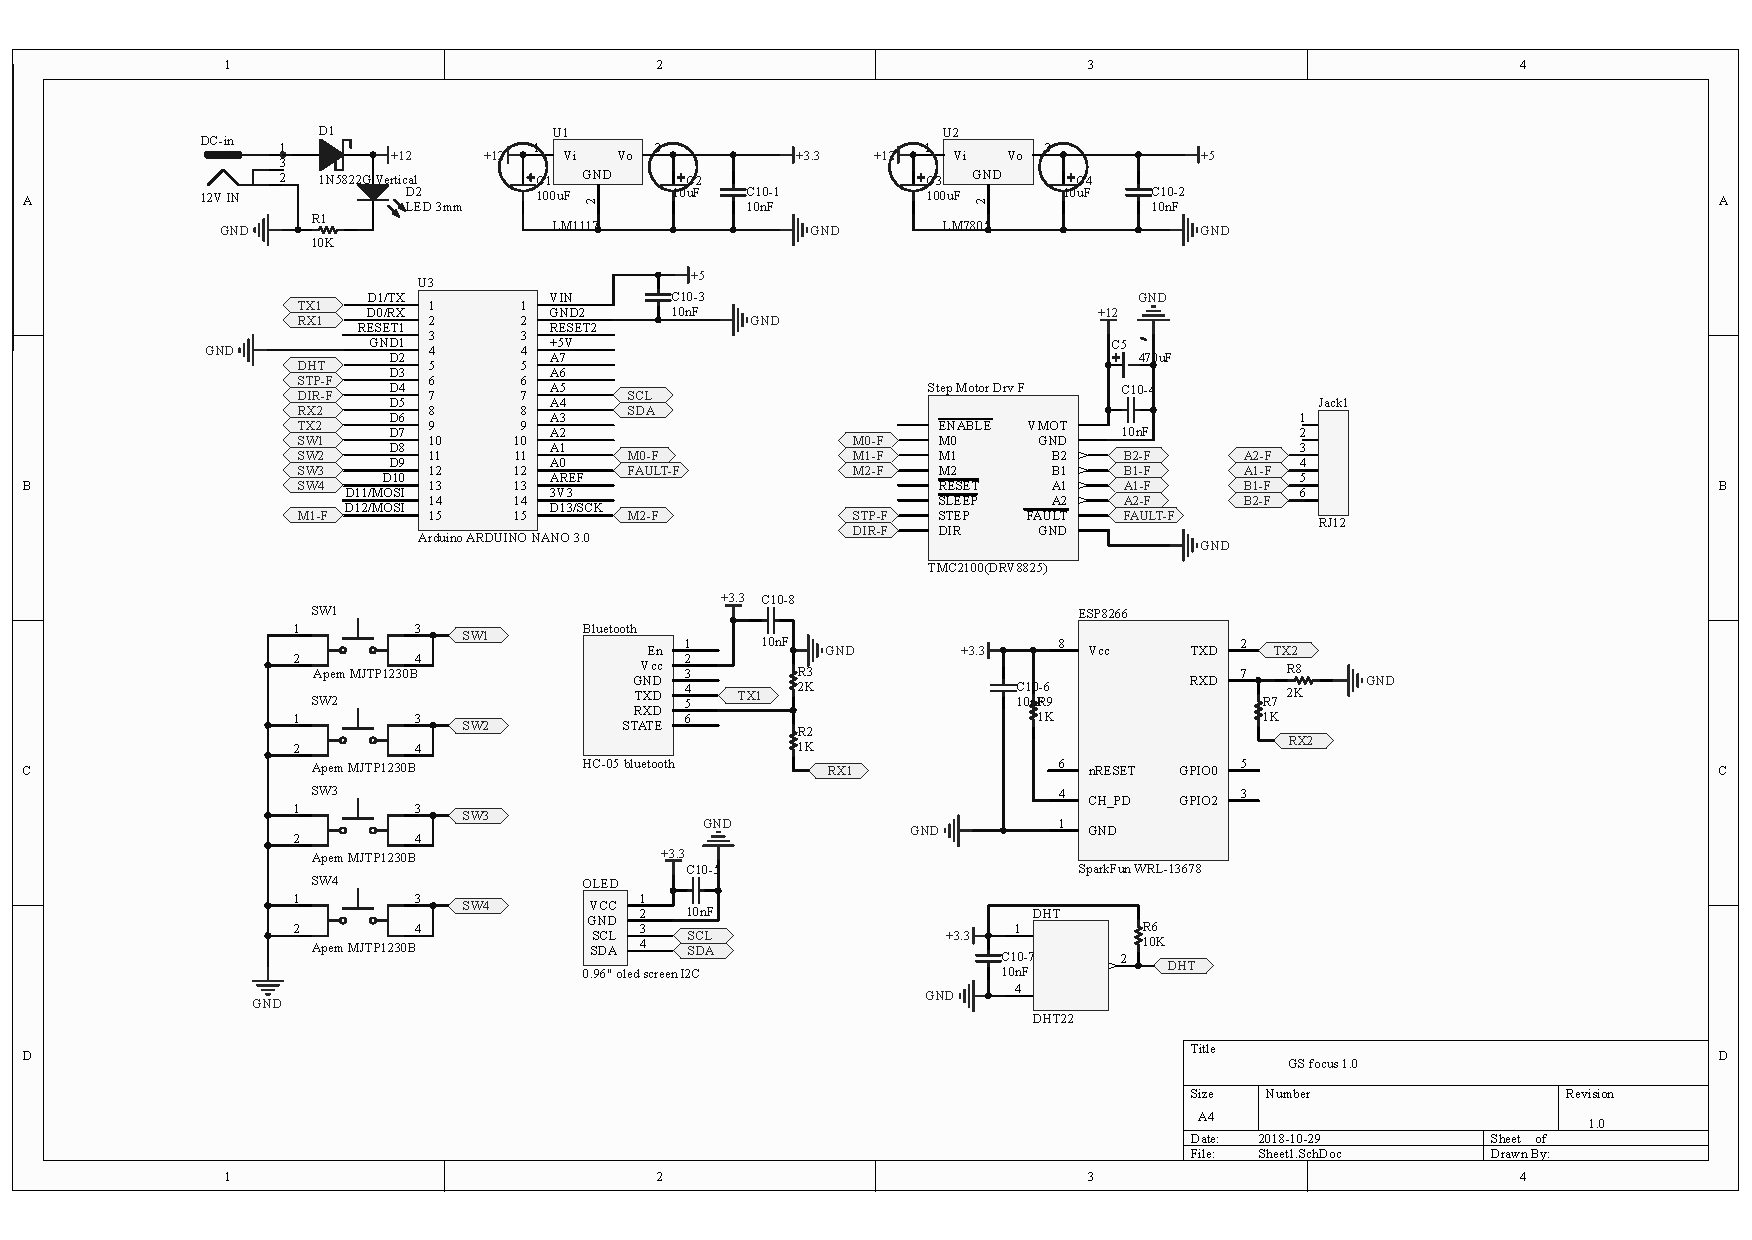
\includegraphics[scale=0.4]{Schematic_Prints}
		\caption{circuitmaker를 이용하여 만든 chart}
		\label{fig:Schematic_Prints}
	\end{figure}
	\begin{figure}[h]
		\centering
		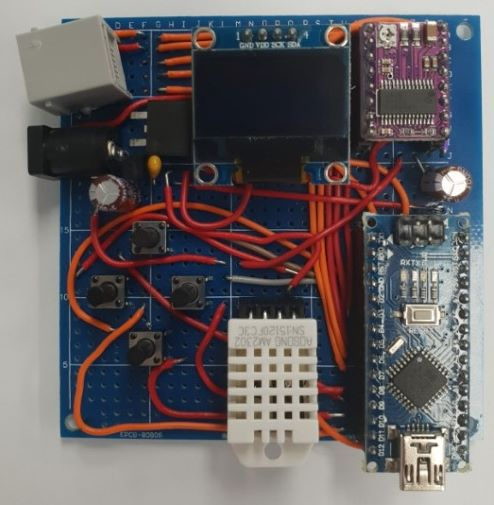
\includegraphics[scale=0.6]{circuit1}
		\caption{만능기판}
		\label{fig:circuit1}
	\end{figure}
	\item 모터 포커서 구동 펌웨어 개발\\
	\begin{figure}[h]
		\centering
		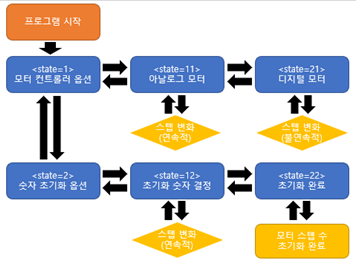
\includegraphics[scale=0.8]{algorithm}
		\caption{알고리즘}
		\label{fig:algorithm}
	\end{figure}
	\begin{figure}[h]
		\centering
		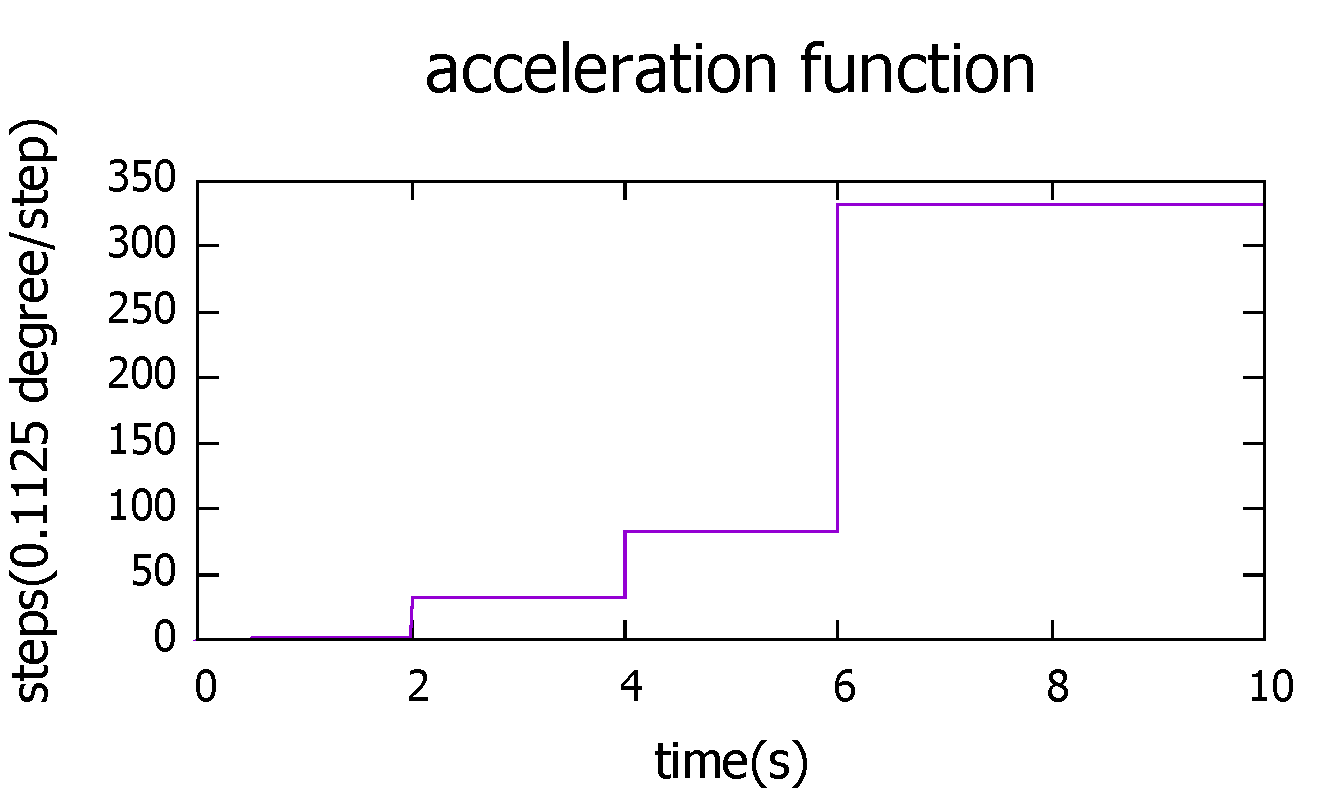
\includegraphics[scale=0.5]{function}
		\caption{가속기능}
		\label{fig:function}
	\end{figure}
	\item ASCOM 드라이버 개발 및 연동\\
	모터 자동 초점 조절 장치를 활용하기 위해서는 컴퓨터와의 연동을 위하여 자동 초점 조절 장치의 ASCOM 드라이버를 C\# 코딩을 이용하여 제작한다. 카메라로부터 정보를 컴퓨터가 받아서 데이터를 분석하고, 이 분석한 데이터를 이용하여 모터에 명령을 내리면 ASCOM 드라이버를 통해 정보를 전달하여 모터 조절이 가능하다.
  \end{itemize}
\end{posterbox}

%% Right Column
\column{0.3\textwidth}
\begin{posterbox}[colbacktitle=purple,coltitle=white,colback=purple!5]{연구 결과의 활용과 기대효과}
자동 초점 조절 장치인 Micro Touch의 경우 가격이 비싸서 부담스러울 수 있고, 제품을 사용하다보면 여러 가지 불편한 점들이 존재하여 실제 천체망원경으로 관측을 할 때에 어려움을 겪을 수 있다. 본 연구에서는 이러한 단점들을 보완하여 다양한 새로운 기능들을 추가하고, arduino 코딩을 기반으로 자동 초점 조절 장치를 개발한다. 이러한 자동 초점 조절 장치가 이용된다면 현재보다 더욱 편리하게 천체망원경의 초점을 맞출 수 있게 되어 천체를 관측하여 사진을 찍을 때 사람의 손보다 수월하게 진행이 가능하다.
\end{posterbox}

\vspace{1em}

\begin{posterbox}[colbacktitle=brown,coltitle=white,colback=brown!5]{추후 연구}
	카메라(또는 CCD) 제어 S/W 개발 및 오토 포커싱 알고리즘 구현\\
	사진 관측을 이용해서 얻은 사진을 컴퓨터로 연결하여 분석이 가능할 수 있도록 카메라(CCD) 제어 시스템을 개발한다. 카메라에 나오는 연속적인 화면의 변화를 실시간으로 보내는 프로그램을 만들어 컴퓨터가 제대로 인식을 하여 모터에 올바른 명령을 내릴 수 있는지 확인한다. 컴퓨터는 이를 자동 초점 조절 장치 컨트롤러에 별의 크기 정보를 알고리즘에 보내준다. 프로그래밍 된 arduino가 모터를 어느 방향으로 돌려야 하는지 판단하여 돌리고, 이 과정을 반복하여 별의 크기가 제일 작아질 때, 즉 별의 초점이 맞을 때 이 과정을 멈춘다. 이러한 과정이 일어나는지 실제로 천체망원경에 달아서 확인한다.
\end{posterbox}

\vspace{1em}

\begin{posterbox}[colbacktitle=yellow,coltitle=black,colback=yellow!5]{References}
	
\bibliography{bibfile} % 참고문헌

\end{posterbox}



\end{columns}
\end{document}

